\section{Optimal Linear Filtering in Mean Square Sense: The Wiener Filter}
\begin{itemize}
    \item Let us consider some important \underline{\textbf{applications}} of the \textbf{LMMSE estimate}.
\[
\textbf{\textcolor{blue}{LMMSE estimator}} \rightarrow
\begin{cases}
\mathbf{\hat{\theta}}_{LMMSE} &= \mathbf{\eta}_{\theta} + \mathbf{C}_{\theta\mathbf{X}}^{T} \mathbf{C}_{\mathbf{X}}^{-1} (\mathbf{X} - \mathbf{\eta}_{\mathbf{X}}) \\
MSE\{\mathbf{\hat{\theta}}_{LMMSE}\} &= \mathbf{C}_{\mathbf{\epsilon}} = \mathbf{C}_{\theta} - \mathbf{C}_{\theta\mathbf{X}}^{T} \mathbf{C}_{\mathbf{X}}^{-1} \mathbf{C}_{\mathbf{X}\theta}
\end{cases}
\]
\item \textbf{\underline{Assumptions}}:
\begin{enumerate}
    \item Observed data = SOI + NOISE, signa and noise are uncorrelated:
    \[
    X[n] = S[n] + W[n], \quad n=0, 1, 2, \dots, N-1 \quad \rightarrow \quad \mathbf{X} = \mathbf{S} + \mathbf{W}
    \]
    \item The signal we want to estimate is a realization of a WSS process, not necessarily Gaussian, with zero mean and known autoc0rrelation function (ACF), i.e known power spectral density (PSD).
    \item The noise is additive, not necessarily Gaussian, not necessarily white, with zero mean and known ACF, i.e. known PSD.
\end{enumerate}
\item From 2 and 3 we obtain that \(\eta_{\theta}=0\) and \(\eta_X =0\), while 1 implies that:
\begin{align*}
&\mathbf{C}_{\mathbf{X}} = E\{\mathbf{X}\mathbf{X}^{T}\} = E\{\mathbf{S}\mathbf{S}^{T}\} + E\{\mathbf{W}\mathbf{W}^{T}\} = \mathbf{C}_{\mathbf{S}} + \mathbf{C}_{\mathbf{W}} \\[8pt]
&\mathbf{\hat{\theta}}_{LMMSE} = \mathbf{C}_{\mathbf{X}\theta}^{T} (\mathbf{C}_{\mathbf{S}} + \mathbf{C}_{\mathbf{W}})^{-1} \mathbf{X} = \mathbf{A}\mathbf{X} \quad \Rightarrow \quad \mathbf{A} = \text{Wiener Smoothing Matrix}
\end{align*}
\item There are various kind of problems that can be solved with the theory of the \textbf{LMMSE estimator} \(\rightarrow\) \underline{\textbf{Wiener Filter}}
\item We have 4 different kinds of \textbf{Wiener Filter},accordin to what is the vector parameter \(\theta\) to be estimated and what are the observed data we use to estimate it:
\[
\textbf{Filtering, Smooting, Prediction , Interpolation}
\]
\begin{figure}[H]
    \centering
    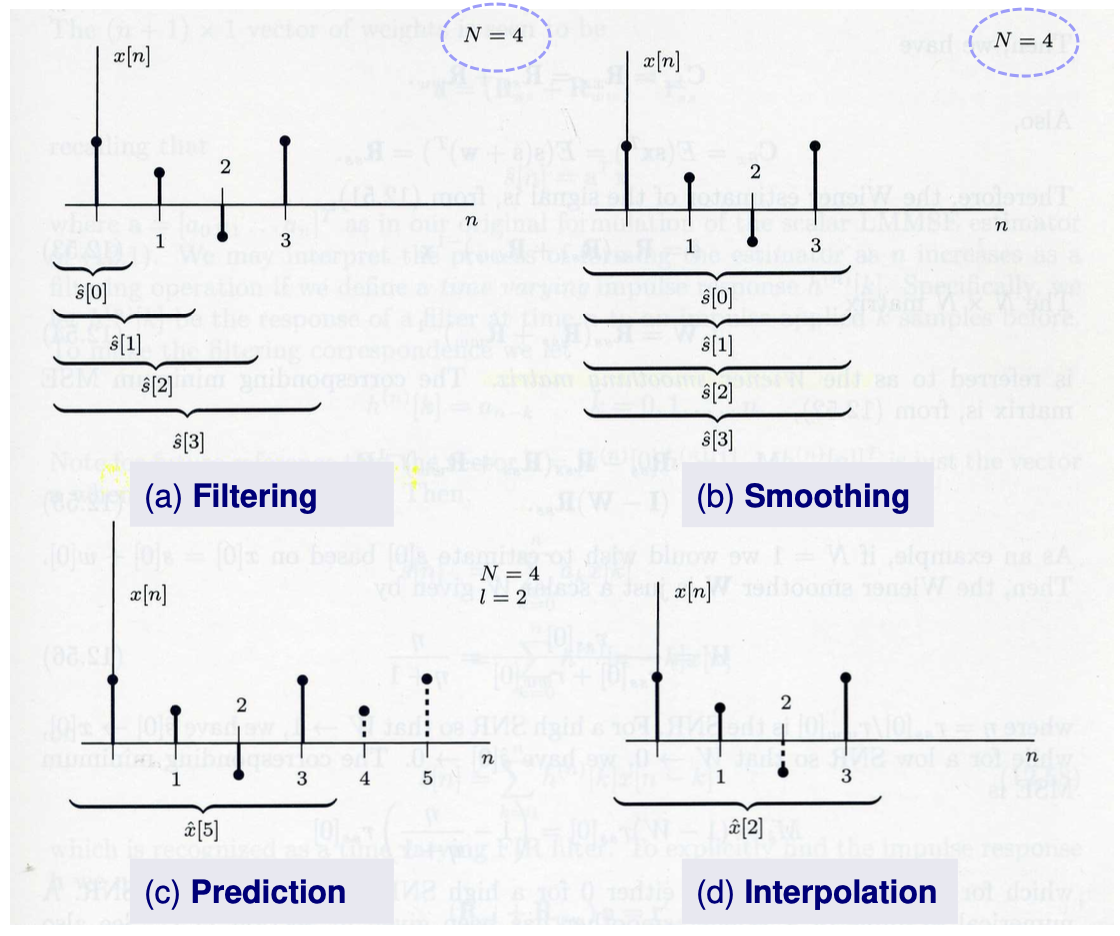
\includegraphics[width=0.65\linewidth]{Image/pdf 9/1.case_4.png}
    \label{fig:placeholder}
\end{figure}
\end{itemize}
\subsection{Smooting Wiener Filter (Batch)}
\begin{itemize}
\item We can say:
\[
\begin{cases}
    \boldsymbol{\theta} = \mathbf{S} = \begin{bmatrix} S[0] & S[1] & \cdots & S[N-1] \end{bmatrix}^T \\[8pt]
    \mathbf{X} = \begin{bmatrix} X[0] & X[1] & \cdots & X[N-1] \end{bmatrix}^T = \mathbf{S} + \mathbf{W} \\[8pt]
    \mathbf{C}_{\mathbf{X}\boldsymbol{\theta}} = \mathbf{C}_{\mathbf{X}\mathbf{S}} = E\{\mathbf{X}\mathbf{S}^T\} = E\{(\mathbf{S} + \mathbf{W})\mathbf{S}^T\} = E\{\mathbf{S}\mathbf{S}^T\} = \mathbf{C}_{\mathbf{S}}
\end{cases}\]
\begin{align*}
&\mathbf{\hat{S}}_{LMMSE} = \mathbf{C}_{\mathbf{S}}(\mathbf{C}_{\mathbf{S}} + \mathbf{C}_{\mathbf{W}})^{-1}\mathbf{X} = \mathbf{A}\mathbf{X} \quad \implies \quad \mathbf{A} = \text{Wiener Smoothing Matrix}\\[10pt]
&\mathbf{C}_{\boldsymbol{\varepsilon}} = \mathbf{C}_{\mathbf{S}} - \mathbf{C}_{\mathbf{S}}(\mathbf{C}_{\mathbf{S}} + \mathbf{C}_{\mathbf{W}})^{-1}\mathbf{C}_{\mathbf{S}} = (\mathbf{I} - \mathbf{C}_{\mathbf{S}}(\mathbf{C}_{\mathbf{S}} + \mathbf{C}_{\mathbf{W}})^{-1})\mathbf{C}_{\mathbf{S}} = (\mathbf{I} - \mathbf{A})\mathbf{C}_{\mathbf{S}}
\end{align*}
    \item The \textbf{Smoothing Wiener filter} working in \textbf{batch mode} is a \textbf{linear time-variant (LTV)} filter, as we will shortly.
    \item The \textbf{Smoothing Wiener Filter} operating in \textbf{batch mode} is a \textbf{linear time-variant (LTV) filter}, since in general the data samples \(\{X[n]\}\)'s are processed with a linear filter whose impulse response chans with discrete-time \(n\).
    \item The case of \textbf{constant signal} is an expection, due to the fact that the signal samples are fully correlated, i.e. \(S[n]=S\) for any \(n\), hence the correlation between \(S[n]\) and the data vector \textbf{X} does not change with time \(n\).
    \item In fact, when the problem is to estimate a constant signal \(S[n]=S\) in additive white noise, we have:
\begin{align*}
&\mathbf{C}_{\mathbf{X}} = \mathbf{C}_{\mathbf{S}} + \sigma_{w}^2 \mathbf{I} \\[8pt]
&C_{\mathbf{S}}[m] = E\{(S[n] - \eta_S)(S[n+m] - \eta_S)\}= E\{(S - \eta_S)^2\} = \sigma_{S}^2 \quad \forall m \\[8pt]
&[\mathbf{C}_{\mathbf{S}}]_{i+1, k+1} = \sigma_{S}^2, \quad i, k = 0, 1, 2, \dots, N-1 
\implies \mathbf{C}_{\mathbf{S}} = \sigma_{S}^2 \mathbf{1}\mathbf{1}^T
\end{align*}

\item Alternatively, the signal covariance matrix can be found as follows:

\begin{align*}
\mathbf{C}_{\mathbf{S}} &= E\{(\mathbf{S} - \boldsymbol{\eta}_{\mathbf{S}})(\mathbf{S} - \boldsymbol{\eta}_{\mathbf{S}})^T\} = E\{(\mathbf{S}\mathbf{1} - \eta_{S}\mathbf{1})(\mathbf{S}\mathbf{1} - \eta_{S}\mathbf{1})^T\} \\[8pt]
&= E\{(S - \eta_{S})^2 \mathbf{1}\mathbf{1}^T\} = E\{(S - \eta_{S})^2\} \mathbf{1}\mathbf{1}^T = \sigma_{S}^2 \mathbf{1}\mathbf{1}^T
\end{align*}
\item hence, the observed data matrix and its inverse are as follows:

\begin{align*}
\mathbf{C}_{\mathbf{X}} &= \mathbf{C}_{\mathbf{S}} + \mathbf{C}_{\mathbf{W}} = \sigma_{s}^2 \mathbf{1}\mathbf{1}^T + \sigma_{w}^2 \mathbf{I} \\[8pt]
&= \sigma_{w}^2 \left( \frac{\sigma_{s}^2}{\sigma_{w}^2} \mathbf{1}\mathbf{1}^T + \mathbf{I} \right) = \sigma_{w}^2 (\gamma \mathbf{1}\mathbf{1}^T + \mathbf{I})\\[8pt]
&\text{where } \gamma \triangleq \frac{\sigma_{s}^2}{\sigma_{w}^2} \quad \text{Signal-to-Noise power Ratio } (SNR)\\[8pt]
&\mathbf{C}_{\mathbf{X}}^{-1} = \frac{1}{\sigma_{w}^2} (\gamma \mathbf{1}\mathbf{1}^T + \mathbf{I})^{-1} = \frac{1}{\sigma_{w}^2} \left( \mathbf{I} - \frac{\gamma}{1+\gamma \mathbf{1}^T \mathbf{1}} \mathbf{1}\mathbf{1}^T \right) \quad \text{Woodbury Identity}
\end{align*}
\item Continuing the derivation:
$$
\boxed{\mathbf{\hat{S}}_{LMMSE} = \mathbf{C}_{\mathbf{S}}(\mathbf{C}_{\mathbf{S}} + \mathbf{C}_{\mathbf{W}})^{-1}\mathbf{X} = \mathbf{A}\mathbf{X} \quad (\eta_{S}=0) \quad \mathbf{A} = \text{Wiener Smoothing Matrix}}
$$
\vspace{-0.25em}
\begin{align*}
\mathbf{\hat{S}}_{LMMSE} &= \mathbf{C}_{\mathbf{S}}(\mathbf{C}_{\mathbf{S}} + \mathbf{C}_{\mathbf{W}})^{-1}\mathbf{X} = \sigma_{s}^2 \mathbf{1}\mathbf{1}^T (\sigma_{s}^2 \mathbf{1}\mathbf{1}^T + \sigma_{w}^2 \mathbf{I})^{-1} \mathbf{X} \\[8pt]
&= \sigma_{s}^2 \mathbf{1}\mathbf{1}^T \left( \frac{1}{\sigma_{w}^2} \left( \mathbf{I} - \frac{\gamma}{1+\gamma \mathbf{1}^T \mathbf{1}} \mathbf{1}\mathbf{1}^T \right) \right) \mathbf{X} = \gamma \mathbf{1}\mathbf{1}^T \left( \mathbf{I} - \frac{\gamma}{1+N\gamma} \mathbf{1}\mathbf{1}^T \right) \mathbf{X} \\[8pt]
&= \gamma \mathbf{1} \left( \mathbf{1}^T - \frac{N\gamma}{1+N\gamma} \mathbf{1}^T \right) \mathbf{X} = \gamma \mathbf{1} \left( 1 - \frac{N\gamma}{1+N\gamma} \right) \mathbf{1}^T \mathbf{X} = \mathbf{1} \frac{N\gamma}{1+N\gamma} \cdot \frac{1}{N} \mathbf{1}^T \mathbf{X} = (\alpha \mathbf{\bar{X}}) \mathbf{1} \\[8pt]
\text{where } \alpha &\triangleq \frac{N\gamma}{1+N\gamma}, \quad \mathbf{\bar{X}} \text{ is the Sample Mean, and } \mathbf{\hat{S}}_{LMMSE} = \alpha \mathbf{\bar{X}}
\end{align*}
\item That is in agreement with what we have already found for \(\eta_s=0\).
\item The \textbf{Wiener smoothing matrix} in this particular case of constant signal is:
\begin{align*}
\mathbf{A} &= \mathbf{C}_{\mathbf{S}}(\mathbf{C}_{\mathbf{S}} + \mathbf{C}_{\mathbf{W}})^{-1} = \mathbf{1}\frac{N\gamma}{1+N\gamma} \cdot \frac{1}{N} \mathbf{1}^T = \frac{\alpha}{N} \mathbf{1}\mathbf{1}^T = \frac{\alpha}{N} \begin{bmatrix} 1 & \cdots & 1 \\ \vdots & \ddots & \vdots \\ 1 & \cdots & 1 \end{bmatrix}_{N \times N}
\end{align*}
$$
\mathbf{\hat{S}}_{LMMSE} = \underbrace{\begin{bmatrix} \hat{S}[0] \\ \hat{S}[1] \\ \vdots \\ \hat{S}[N-1] \end{bmatrix}}_{N \times 1} = \frac{\alpha}{N} \begin{bmatrix} 1 & \cdots & 1 \\ \vdots & \ddots & \vdots \\ 1 & \cdots & 1 \end{bmatrix} \begin{bmatrix} X[0] \\ X[1] \\ \vdots \\ X[N-1] \end{bmatrix} = \begin{bmatrix} \hat{S}_{LMMSE} \\ \hat{S}_{LMMSE} \\ \vdots \\ \hat{S}_{LMMSE} \end{bmatrix} = \hat{S}_{LMMSE} \mathbf{1}
$$

\item Hence, in the case of completely correlated signal \(S[n]=S\) embedded in white noise \(W[n]\), all the data \(\{X[n]\}\) are weighted in the same way, whatever is the discrete-time \(n\), since all the rows of the matrix \textbf{A} are equal.
\item In the more general of \textbf{partially correlated signal}, the rows of the Wiener smoothing matrix are no more all equal and hence the matrix represents a \textbf{linear time-variant filter (LTV)}:
\begin{align*}
&\mathbf{\hat{S}}_{LMMSE}
=
\underbrace{\begin{bmatrix}
    \hat{S}[0] \\
    \hat{S}[1] \\
    \vdots \\
    \hat{S}[N-1]
\end{bmatrix}}_{N\times1}
= \underset{N \times N}{\mathbf{A}} \cdot \underset{N \times 1}{\mathbf{X}}
=
\begin{bmatrix}
    \mathbf{a}_0 \\
    \mathbf{a}_1 \\
    \vdots \\
    \mathbf{a}_{N-1}
\end{bmatrix}
\begin{bmatrix}
    X[0] \\
    X[1] \\
    \vdots \\
    X[N-1]
\end{bmatrix}\\[8pt]
&\text{where } \mathbf{a}_n \text{ is the } (n+1)\text{-th row of matrix } \mathbf{A}, \text{ i.e.}\\[8pt]
&\underbrace{\mathbf{a}_n}_{1\times N} \triangleq \begin{bmatrix} a_{n,0} & a_{n,1} & \cdots & a_{n,N-1} \end{bmatrix}, \quad n = 0, 1, 2, \dots, N-1
\end{align*}
\item We can obtain \(\hat{S}[n]\):
\begin{align*}
\mathbf{\hat{S}}[n] &= \mathbf{a}_n \mathbf{X} = \begin{bmatrix} a_{n,0} & a_{n,1} & \cdots & a_{n,N-1} \end{bmatrix}
\begin{bmatrix}
    X[0] \\
    X[1] \\
    \vdots \\
    X[N-1]
\end{bmatrix}\\[8pt]
&= \sum_{k=0}^{N-1} a_{n,k} X[k] = \sum_{k=0}^{N-1} h[k,n] X[k] \neq \sum_{k=0}^{N-1} h[n-k] X[k], \quad n = 0, 1, 2, \dots, N-1 \\[8pt]
&\text{where } h[k,n] \triangleq a_{n,k} \text{ is the impulse response at discrete-time } n
\end{align*}
\item In general the rows of matrix \textbf{A} are not equal. This implies that the impulse response of the \textbf{smoothin Wiener filter} operating in \textbf{batch mode} changes with the discrete-time \(n\), i.e. it is time-variant.

\item This is due to the fact that the correlation of the signal sample \(S[n]\) with the data vector \textbf{X} changes with time \(n\). This is true in particular for the first \(L_S\) samples and the last \(L_S\) samples of signal vector \textbf{S}, where \(L_S\) is the correlation length of process \(S[n]\).
\begin{figure}[H]
    \centering
    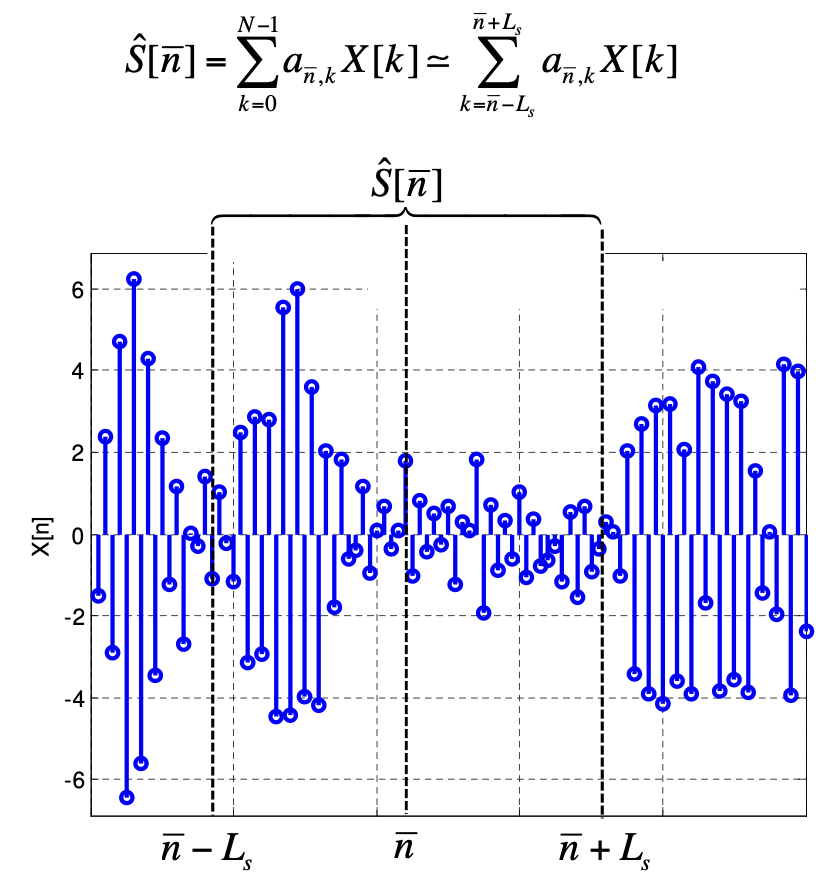
\includegraphics[width=0.4\linewidth]{Image/pdf 9/2.Graph_1.png}
    \label{fig:placeholder}
\end{figure}
\begin{figure}[H]
    \centering
    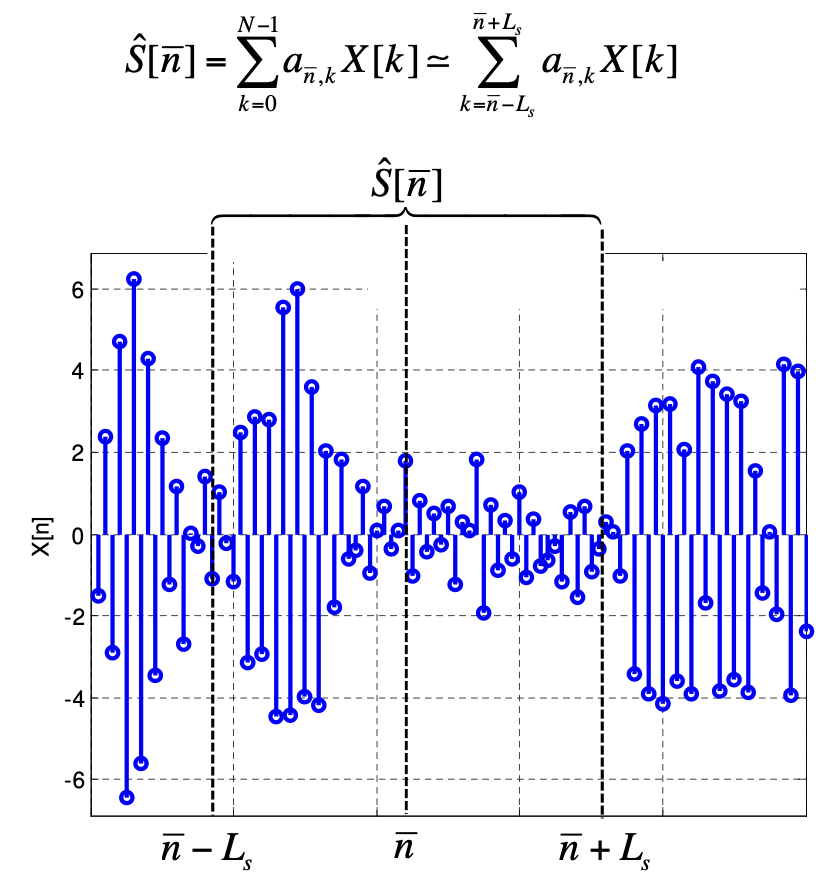
\includegraphics[width=0.4\linewidth]{Image/pdf 9/2.Graph_1.png}
    \label{fig:placeholder}
\end{figure}
\begin{figure}[H]
    \centering
    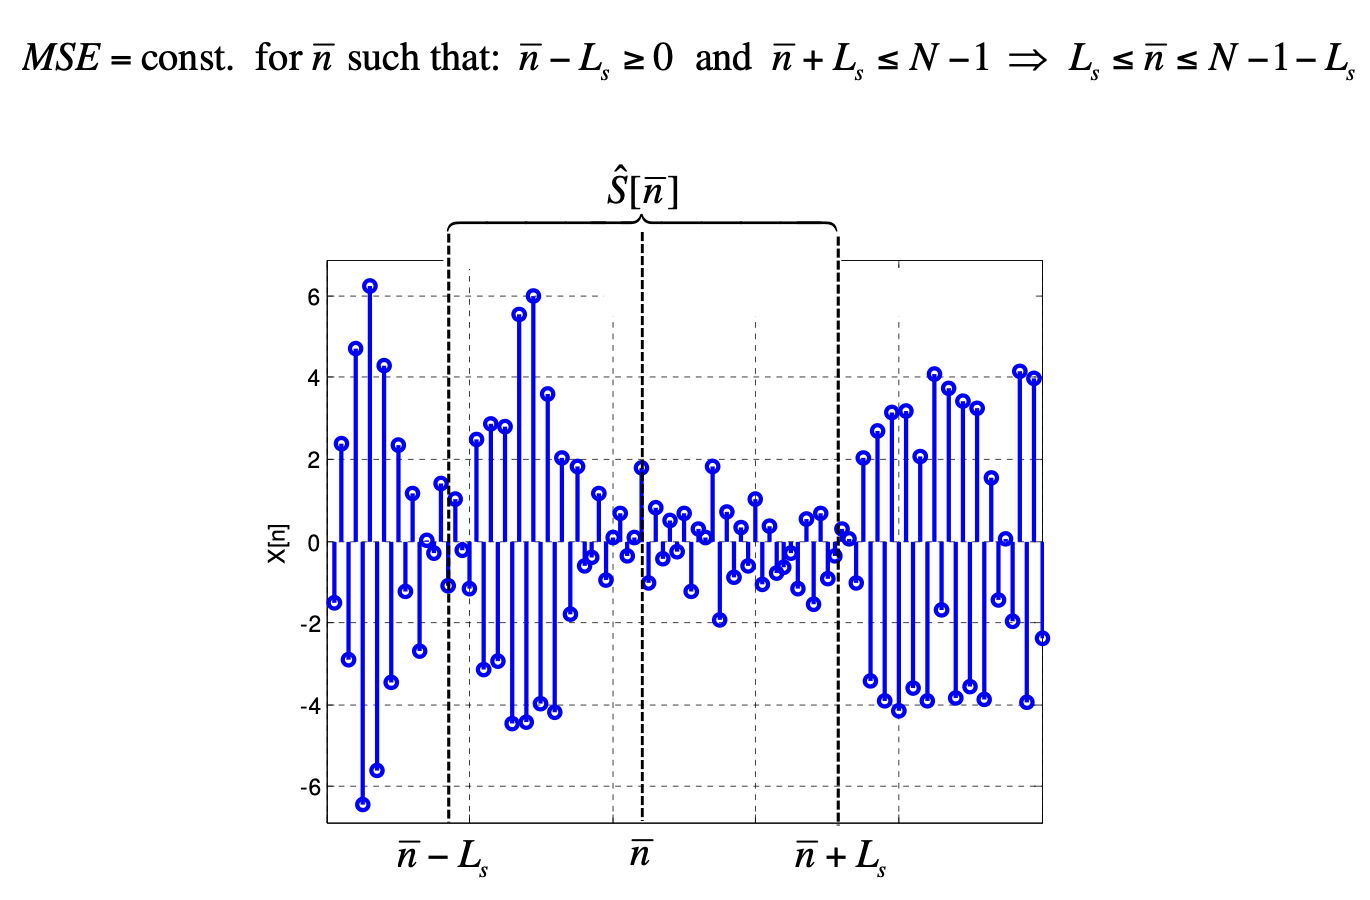
\includegraphics[width=0.65\linewidth]{Image/pdf 9/3.Graph_2.png}
    \label{fig:placeholder}
\end{figure}
\begin{figure}[H]
    \centering
    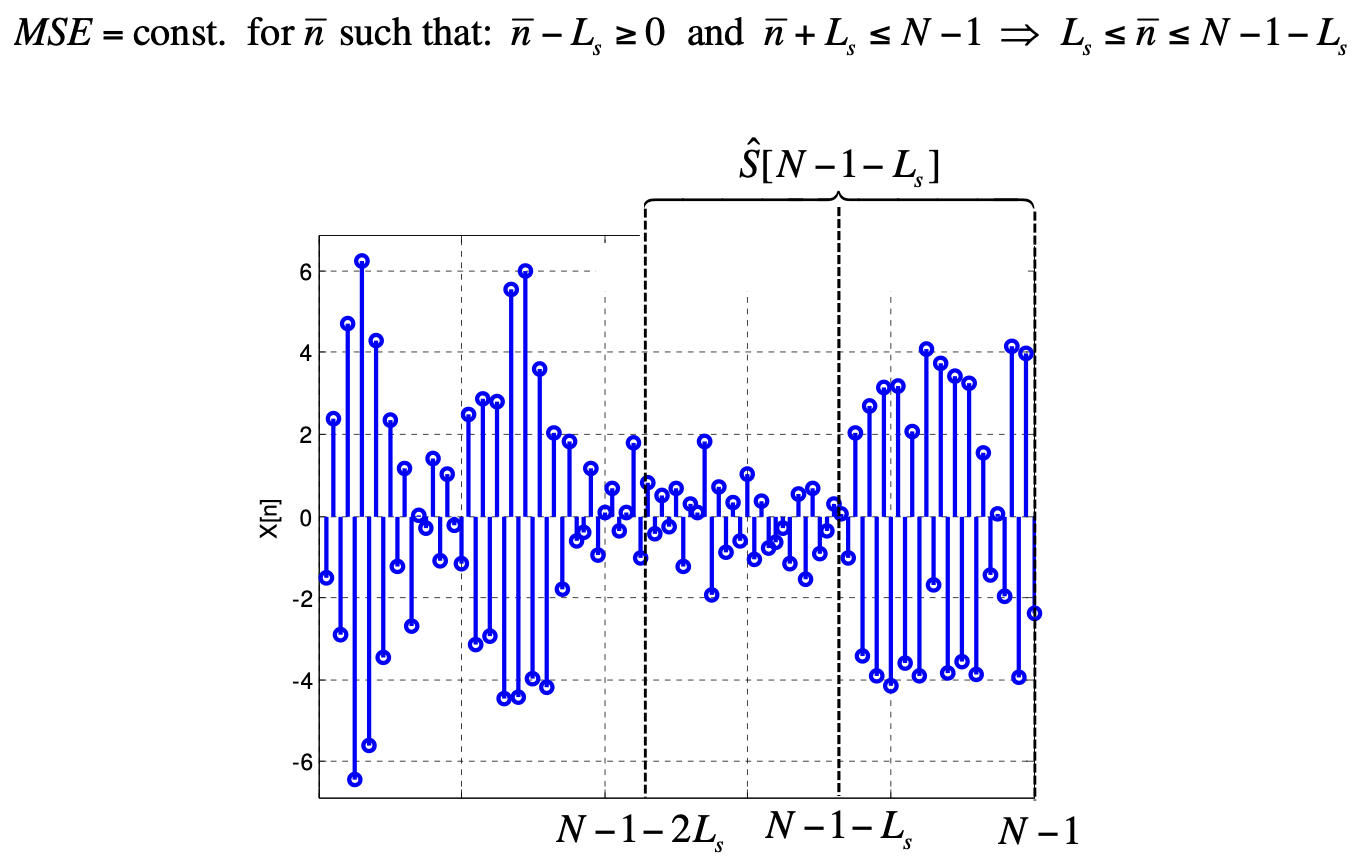
\includegraphics[width=0.65\linewidth]{Image/pdf 9/4.Graph_3.png}
    \label{fig:placeholder}
\end{figure}
\begin{figure}[H]
    \centering
    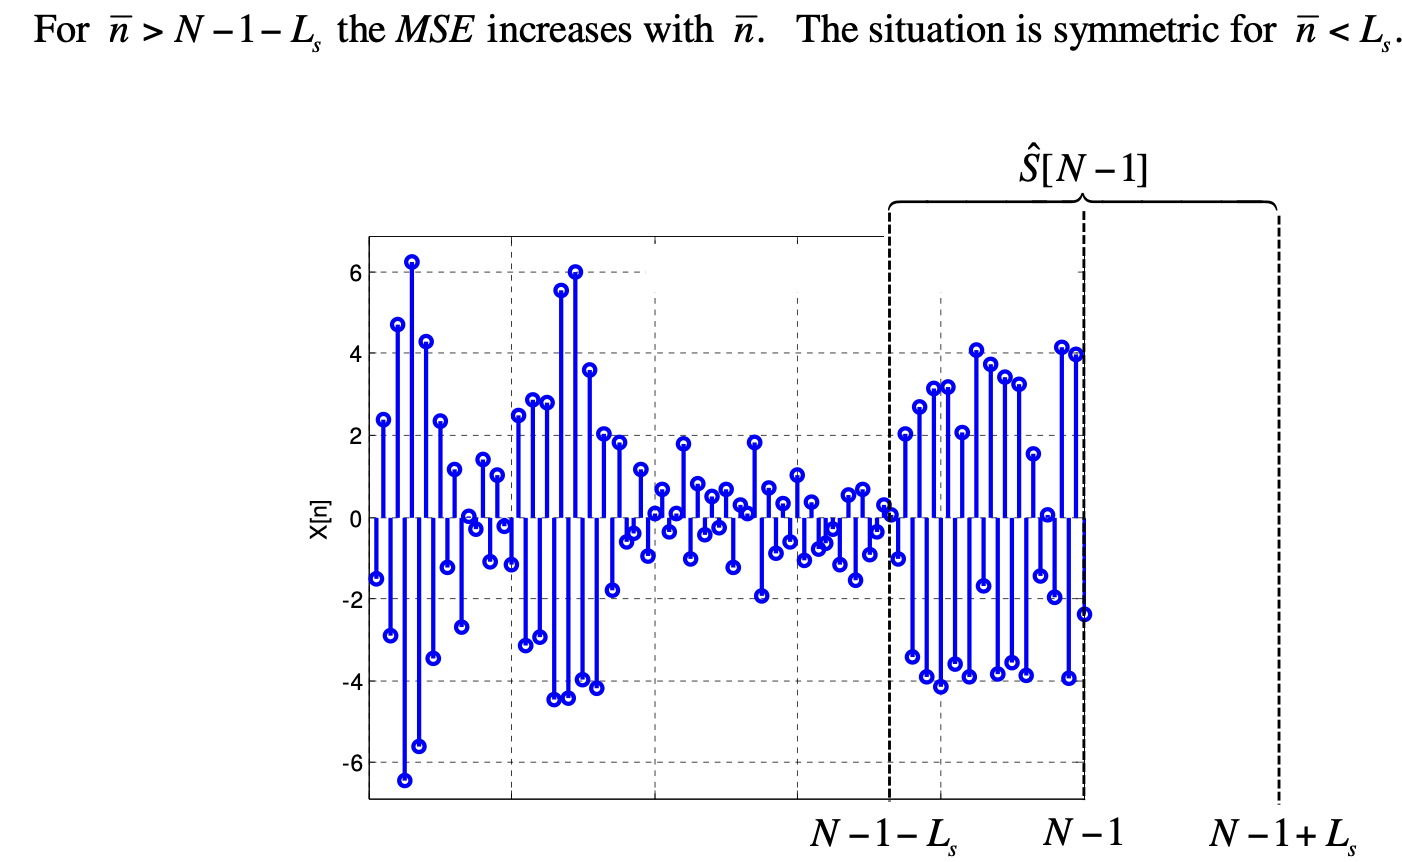
\includegraphics[width=0.65\linewidth]{Image/pdf 9/5.graph_4.png}
    \label{fig:placeholder}
\end{figure}
(ESEMPIO NUMERICO 9, SLIDE 16-24)
\end{itemize}
\subsection{Wiener Filter (sequential)}
\begin{itemize}
    \item When the signal and noise processes are WSS, we can enforce the \textbf{Wiener Filter} to be not only \textbf{linear} but also \textbf{time-invariant}, i.e. \textbf{LTI}, so the estimate is made available \textbf{sequentially} at the output of the filter:
    \begin{figure}[H]
        \centering
        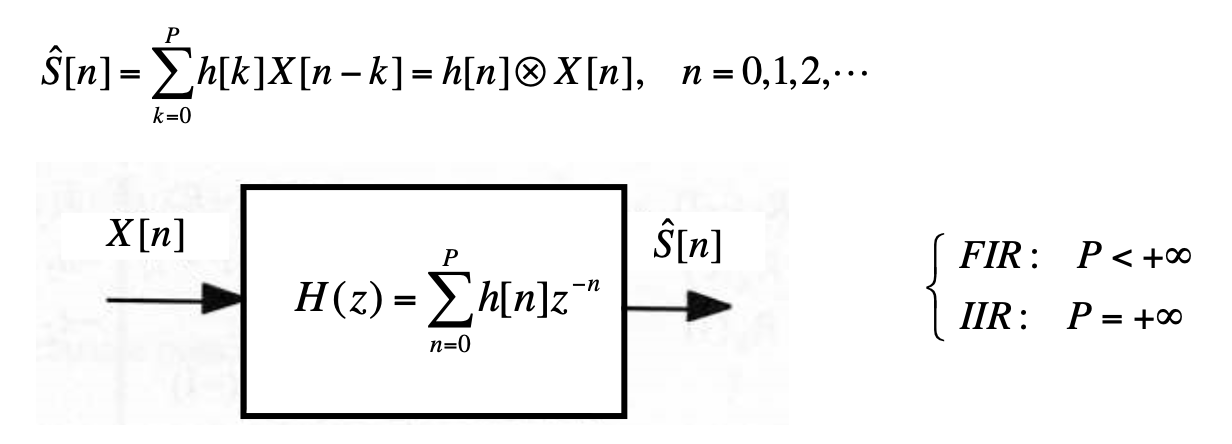
\includegraphics[width=0.65\linewidth]{Image/pdf 9/Screenshot 2025-12-14 at 6.25.24 PM.png}
        \label{fig:placeholder}
    \end{figure}
\end{itemize}



\clearpage